%!TEX root = ../thesis.tex
\chapter{Evaluation}
\label{ch:Evaluation}
\section{Datensammlung und Grundlage}
{ \label{sec:datengrundlage}
	Die Datengrundlage zur Analyse bilden Videos im MP4 Format in der Auflösung 1920 \texttimes 1080 Pixeln. Diese wurden an der Autobahnbrücke zur A1 in Münster-Nienberge aufgenommen \citep{GMaps}. Das Wetter war bedeckt, somit konnte die Sonne nicht einzelne Objekte überstrahlen. Das Videomaterial mit dem evaluiert wurde, stammt vom 17.07.2023 und wurde mittags (12:53 Uhr) aufgenommen. Es zeigt primär die beiden Fahrspuren der Autobahn (siehe Abb. \ref{Bsp_Evaluations_Vidmat}). \\
	Am unteren Rand ist im Vordergrund rechts das Geländer der Autobahnbrücke zu erkennen. Links unten im Bild ist ein Warnkegel zu sehen. Der mittlere Bereich des Bildes wird von den Fahrspuren dominiert, rechts mittig sind zwei Verkehrsschilder. Im Hintergrund ist ein weiteres Verkehrsschild zu erkennen, welches über die sich vom Betrachter entfernende führende Fahrspur ragt. An den Seiten der beiden Fahrspuren sind Bäume. \\
	Das Videomaterial wurde mit der Software DaVinci Resolve \citep{davinciresolve} geschnitten um die für die Evaluation wichtige Vergleichbarkeit und Frameanzahl zu erhalten.
	\begin{figure}[ht]
		\centering
		\includegraphics*[scale = 0.35, keepaspectratio ]{images/Evaluation/Screenshot_Video_A10s.png}
		\caption[Beispielframe aus Videomaterial]{Beispielframe aus Videomaterial (Quelle: eigene Darstellung)} 
		\label{Bsp_Evaluations_Vidmat}
 \end{figure}
}


\section{Testumgebung}{
	Das Testsystem besteht aus einem Lenovo Thinkpad P14s. Dieses besitzt einen AMD Ryzen 7 PRO 5850U Prozessor mit 8 Kernen und 16 Threads bei einem Basistakt von 1,9 GHz und einem Höchsttakt von 4,4 GHz. Die integrierte Grafikeinheit AMD Radeon Graphics Einheit kann auf 8 GB VRAM zugreifen, sodass der effektive verfügbare Arbeitsspeicher des Systems bei 39,8 GB liegt \citep{PSREF21}. Die Entwicklungsumgebung 'Visual Studio Code' ist auf einer 64-bit Windows 11 Pro Installation in der Version 22H2 installiert. Für Details in der Python Konfiguration siehe Kap. \ref{sec:Python}. Für die Testdurchläufe ist der Laptop an ein 65 Watt Netzteil angeschlossen, um ein Throttling der CPU zu verhindern.
}
\section{Einstellungen und Testdatensätze}
{% \begin{itemize}
	% 	\item Evaluation mit verschiedenen Testvideos
	% 	\item immer das gleiche Video nur mit verschiedenen Längen
	% 	\item Dann verschiedene Berechnungsmethode (YOLO every frame, yolo result)
	% 	\item mit und ohne schwarzes video ?
	% 	\item mit verschiedenen YOLO Modellen (v8n, v8x, v8)
	% \end{itemize}
	Es werden 2 Videodaten genommen, die sich jeweils in der Länge unterscheiden. Beide Testdatensätze basieren auf dem gleichen Video. Die Länge unterscheidet sich, da das erste Video 1 Sekunde, bzw. 30 Frames, lang ist und das zweite Video 10 Sekunden dauert, bzw. 300 Frames besitzt. Hier überschneidet sich die erste Sekunde. \\
	Es werden 3 YOLO Modelle benutzt: YOLO8n, YOLOv8n (small), YOLOv8m (medium) und YOLOv8x (extra large). Diese sind mit verschieden großen Datensätzen trainiert worden, für Details siehe Kapitel \ref{subsec:YOLOv8_theoretic}.
	Die Einstellungen des Programms für die Grenze der Punktsubstitution der DCE sind, dass Autos auf 10 Punkte, Motorräder auf 5 und Lkw auf 8 Punkte reduziert werden.
	% \begin{itemize}
	% 	\item Car: 10
	% 	\item Motorcycle: 5
	% 	\item Truck: 8
	% 	\item other Object: 20
	% \end{itemize}
	Objekte, welche nicht den drei Hauptklassen entsprechen werden pauschal auf 20 Punkte vereinfacht. Das Video wird  schwarz gerendert, sodass sich nur weiße Polygone im Video bewegen. Außerdem werden für jedes Polygon die detektierte Klasse und der Confidence Score in jedem Frame angezeigt.

}
\section{Ergebnisse\label{sec:Ergebnisse}}  
\todo{Tabellen bei >1000 Zahlen mit 1.000 ausfüllen (Punkt zur Trennung)}
{Die Winkelabweichung der einzelnen Polygone zueinander wird mit verschiedenen Methoden  (siehe Kap. \ref{py:Shape_Sim_Meas}) berechnet. Es wird zunächst auf die allgemeinen Ergebnisse ohne Klassenunterscheidung eingegangen und danach werden die Ergebnisse mit Klassenunterscheidung erläutert. Ein Beispielframe aus dem 10-sekündigen Datensatz ist in Abb. \ref{Bsp_ErgebRVA10s_Vidmat} zu sehen.\\
Alle Angaben in den Tabellen, außer bei den absoluten Anzahlen und in Tab. \ref{tab:YOLO8_A1s_A10s_Comp}, sind in Grad (Deg.). Die Modelle von YOLO werden mit 8n, 8m, 8x entsprechend abgekürzt und werden immer in der Version \glqq -seq\grqq{} genutzt.}
\begin{figure}[ht]
	\centering
	\includegraphics*[scale = 0.35, keepaspectratio ]{images/Evaluation/Screenshot_A10s_RV.png}
	\caption[Beispielframe aus mit der direkten YOLO Anwendung analysiertem Videomaterial]{Beispielframe aus mit der 2. YOLO Implementierung analysiertem Videomaterial (Quelle: eigene Darstellung)} 
	\label{Bsp_ErgebRVA10s_Vidmat}
\end{figure}
\subsection{Winkelabweichung ohne Klassenunterscheidung}
{	\todo{klare Benennung von YOLO oder Yolo; bzw. Yolov8n oder 8n etc.}
	\todo{Yolo Modelle ebenfalls durchgehend klar benennen}
	In der Tabelle \ref{tab:YOLO8_A1s} sind die durchnittlichen Winkelabweichungen pro Polygon und pro Winkel zu sehen. Diese Abweichung wurde über das gesamte Video berechnet für alle Polygone ohne Klassenunterscheidung berechnet.  EFV steht für die 1. YOLO Version, in der jeder Frame extrahiert wird (siehe Kap. \ref{py:YOLO_every_frame}) und RV für die 2. YOLO Version (siehe Kap. \ref{py:YOLO_res_vers}), wo YOLO zuerst das Video insgesamt analysiert. Beide Implementierungen unterscheiden sich von den statistischen Auswertungen nur marginal.\\
	Es ist auffällig, dass die durchschnittliche  Winkelabweichung steigt, je größer der Trainingsdatensatz des verwendeten Modells ist. Dies könnte daran liegen, dass bei einem größeren Trainingsdatensatz mehr Detektionen möglich sind, welche damit  die Abweichung erhöhen. Auch an dem steigenden Wert der absoluten Abweichung ist zu sehen, dass es Unterschiede zwischen den Modellen gibt. Die absolute Winkelabweichung steigt insbesondere im Vergleich von 8n mit 3910,4 Grad (RV Version) zu 8m mit 7358,55 Grad (RV Version) ebenfalls an. Dies ist auch im Vergleich zu 8x zu sehen. \\
	Die erkannte Punktanzahl nach der Vereinfachung mit der DCE bleibt relativ konstant zwischen den Modellen, abgesehen von den Punkten bei 8m. Dies ist damit zu erklären, dass die Vereinfachung mit der DCE zu konstanten und gleich bleibenden Punkt- und Polygonanzahlen führt. \\
	Der Unterschied zwischen 8n und 8m ist auch in der Zahl der verglichenen Polygone sichtbar. Dieser Wert gibt an, wie viel Polygone mit gleicher Klasse verglichen zum nächsten Frame in die Berechnung der absoluten Abweichung einfließen. Es wurden bei der Berechnung der absoluten Abweichung die Differenzen zwischen dieser Anzahl an Polygonen summiert. Im Vergleich zu 8m und 8x ergibt sich nur eine gering ansteigende Zahl verglichener und erkannter Polygone. \\
	Die Prozessierungszeit steigt mit der Verwendung komplexerer YOLO Modelle an. Im Vergleich zwischen den Implementierungen ist zu erkennen, dass die zweite Variante performanter ist.
	\begin{table}[h]
		\centering
	\caption[Vergleich der verschiedenen YOLO Modelle bei 1 Sekunde Video (30 Frames) (Quelle: eigene Darstellung)]{Vergleich der verschiedenen YOLO8 bei 1 Sekunde Video (30 Frames) (Quelle: eigene Darstellung; \ref{cd:listing_A1s_EF_results.txt(Y8n)}; \ref{cd:listing_A1s_RV_results.txt(Y8n)}; \ref{cd:listing_A1s_EF_results.txt(Y8m)}; \ref{cd:listing_A1s_RV_results.txt(Y8m)}; \ref{cd:listing_A1s_EF_results.txt(Y8x)}; \ref{cd:listing_A1s_RV_results.txt(Y8x)})}
	\label{tab:YOLO8_A1s}
	\begin{tabular}{l|l|l|l|l|l|l}
		& \textbf{8n (EFV)} & \textbf{8n (RV)} & \textbf{8m (EFV)} & \textbf{8m (RV)} & \textbf{8x (EFV)} & \textbf{8x (RV)} \\ \hline
	   \textit{\begin{tabular}[c]{@{}l@{}}Durchschn. Abweichung\\ p. Polygon (in Deg.)\end{tabular}} & 26,49 & 26,97 & 35,19 & 35,04 & 44,33 & 48,12 \\ \hline
	   \textit{\begin{tabular}[c]{@{}l@{}}Durchschn. Abweichung  \\ p. Winkel (in Deg.)\end{tabular}} & 2,04 & 2,09 & 3,59 & 3,56 & 5,05 & 5,46 \\ \hline
	   \textit{} &  &  &  &  &  &  \\ \hline
	   \textit{\begin{tabular}[c]{@{}l@{}}absolute Abweichung  \\ (in Deg)\end{tabular}} & 3894,53 & 3910,4 & 7354,98 & 7358,55 & 9398,12 & 10298,28 \\ \hline
	   \textit{erkannte Punkte/Winkel} & 1912 & 1873 & 2050 & 2065 & 1860 & 1885 \\ \hline
	   \textit{erkannte Polygone} & 147 & 145 & 209 & 210 & 212 & 214 \\ \hline
	   \textit{verglichene Polygone} & 131 & 129 & 188 & 189 & 193 & 194 \\ \hline
	   \textit{\begin{tabular}[c]{@{}l@{}}Prozessierungszeit\\ (in Sek.)\end{tabular}} & 92,52 & 81,51 & 111,6 & 100,03 & 134,9 & 102,46
	   \end{tabular}
	\end{table}
	\begin{table}[h]
		\centering
		\caption[Vergleich der verschiedenen YOLO8 bei 10 Sekunde Video (300 Frames) (Quelle: eigene Darstellung)]{Vergleich der verschiedenen YOLO8 bei 10 Sekunde Video (300 Frames) (Quelle: eigene Darstellung; \ref{cd:listing_A10s_EF_results.txt(Y8n)}; \ref{cd:listing_A10s_RV_results.txt(Y8n)}; \ref{cd:listing_A10s_EF_results.txt(Y8m)}; \ref{cd:listing_A10s_RV_results.txt(Y8m)}; \ref{cd:listing_A10s_EF_results.txt(Y8x)}; \ref{cd:listing_A10s_RV_results.txt(Y8x)})}
		\label{tab:YOLO8_A10s}
		\begin{tabular}{l|l|l|l|l|l|l}
		& \textbf{8n (EFV)} & \textbf{8n (RV)} & \textbf{8m (EFV)} & \textbf{8m (RV)} & \textbf{8x (EFV)} & \textbf{8x (RV)} \\ \hline
		\textit{\begin{tabular}[c]{@{}l@{}}Durchschn. Abw.\\ p. Polygon (in Deg.)\end{tabular}} & 53,07 & 53,11 & 49,76 & 49,79 & 57,93 & 58,04 \\ \hline
		\textit{\begin{tabular}[c]{@{}l@{}}Durchschn. Abw.  \\ p. Winkel (in Deg.)\end{tabular}} & 4,29 & 4,29 & 5,21 & 5,21 & 6,59 & 6,6 \\ \hline
		\textit{} &  &  &  &  &  &  \\ \hline
		\textit{\begin{tabular}[c]{@{}l@{}}absolute Abw. \\ (in Deg)\end{tabular}} & 73.075,23 & 73.075,23 & 100.561,26 & 100.579,53 & 122.111,04 & 122.133,17 \\ \hline
		\textit{erk. Punkte/Winkel} & 17.043 & 17.042 & 19.298 & 19.298 & 18.534 & 18.498 \\ \hline
		\textit{erk.  Polygone} & 1.377 & 1.376 & 2.021 & 2.020 & 2.108 & 2.104 \\ \hline
		\textit{\begin{tabular}[c]{@{}l@{}}verglichene\\ Polygone\end{tabular}} & 1.235 & 1.234 & 1.871 & 1.870 & 1.964 & 1960 \\ \hline
		\textit{\begin{tabular}[c]{@{}l@{}}Prozessierungszeit\\ (in Min.)\end{tabular}} & 23,56 & 22,16 & 26,39 & 22.25 & 28,48 & 23,84
		\end{tabular}
	\end{table}



	Wenn man nun die Tabelle \ref{tab:YOLO8_A1s_A10s_Comp} betrachtet, ist zu sehen, dass die durchschnittliche Abweichung pro Polygon und Winkel sich ungefähr verdoppelt hat, wenn die Anzahl der Frames verzehnfacht wird. Dies geht einher mit einer ca. 18-fachen Steigerung der absoluten Abweichung im Vergleich von Tabelle \ref{tab:YOLO8_A1s} zu Tabelle \ref{tab:YOLO8_A10s} bei YOLOv8n. Dabei ist die Anzahl der Punkte, der erkannten Polygone und der verglichenen Polygone um das ca. 9-fache gestiegen, während die Prozessierungszeit bei 8n um das 15-fache anstieg. \\
	Bei Verwendung der größeren YOLO Modelle verringert sich der Anstieg der absoluten Abweichung. Dies ist auch an den absoluten Zahlen in Tabelle \ref{tab:YOLO8_A1s} und \ref{tab:YOLO8_A10s} zu sehen, die bei diesen Modellen bei beiden Videos stark ansteigen. Die Zahl der erkannten Punkte/Winkel und Polygone ist relativ gleichbleibend, während bei der Zahl der verglichenen Polygone ein leichter Anstieg zu sehen ist. Dies kann mit genauerer Klassifizierung durch die größeren Trainingsdatensätze der YOLO Modelle zusammenhängen. \\
	Die Prozessierungszeit sinkt jedoch im Verhältnis zur steigenden Framezahl mit den größeren Modellen langsam ab.

	\begin{table}[ht]
		\centering
	\caption[Anstieg der verschiedenen YOLO8 Modelle im Vergleich von  1 Sekunde Video (30 Frames) zu 10 Sekunden Video (300 Frames) als Faktor]{Anstieg der verschiedenen YOLO Modelle im Vergleich von  1 Sekunde Video (30 Frames) zu 10 Sekunden Video (300 Frames) als Faktor (Quelle: eigene Darstellung; \ref{cd:listing_A1s_EF_results.txt(Y8n)}-\ref{cd:listing_A1s_RV_results.txt(Y8x)} )}
	\label{tab:YOLO8_A1s_A10s_Comp}
	\begin{tabular}{l|l|l|l|l|l|l}
	& \textbf{8n (EFV)} & \textbf{8n (RV)} & \textbf{8m (EFV)} & \textbf{8m (RV)} & \textbf{8x (EFV)} & \textbf{8x (RV)} \\ \hline
	\textit{\begin{tabular}[c]{@{}l@{}}Anstieg Durchschn. \\ Abweichung p. Polygon\end{tabular}} & 2,02 & 1,97 & 1,85 & 1,42 & 1,31 & 1,21 \\ \hline
	\textit{\begin{tabular}[c]{@{}l@{}}Anstieg Durchschn.\\ Abweichung p. Winkel\end{tabular}} & 2,10 & 2,05 & 1,45 & 1,46 & 1,30 & 1,21 \\ \hline
	\textit{} &  &  &  &  &  &  \\ \hline
	\textit{\begin{tabular}[c]{@{}l@{}}Anstieg absolute\\ Abweichung\end{tabular}} & 18,76 & 18,68 & 13,67 & 13,67 & 12,99 & 11,86 \\ \hline
	\textit{\begin{tabular}[c]{@{}l@{}}Anstieg erkannte\\ Punkte/Winkel\end{tabular}} & 8,91 & 9,09 & 9,41 & 9,35 & 9,96 & 9,81 \\ \hline
	\textit{\begin{tabular}[c]{@{}l@{}}Anstieg erkannte\\ Polygone\end{tabular}} & 9,37 & 9,48 & 9,66 & 9,62 & 9,94 & 9,83 \\ \hline
	\textit{\begin{tabular}[c]{@{}l@{}}Anstieg verglichene\\ Polygone\end{tabular}} & 9,43 & 9,56 & 9,95 & 9,90 & 10,18 & 10,10 \\ \hline
	\textit{\begin{tabular}[c]{@{}l@{}}Anstieg \\ Prozessierungszeit\end{tabular}} & 15,28 & 16,31 & 14,19 & 13,35 & 12,66 & 13,96
	\end{tabular}
	\end{table}
} 
%\clearpage
	\subsection{Winkelabweichung mit Klassenunterscheidung}
	{
		
	\begin{table}[ht]
		\centering
		\caption[Vergleich der SSMs bei verschiedenen YOLO8 bei 1 Sekunde Video (30 Frames)]{Vergleich der SSMs bei verschiedenen YOLO Modellen bei 1 Sekunde Video (30 Frames) (Alle Angaben in Grad) (Quelle: eigene Darstellung; \ref{cd:listing_A1s_EF_results.txt(Y8n)}; \ref{cd:listing_A1s_RV_results.txt(Y8n)}; \ref{cd:listing_A1s_EF_results.txt(Y8m)}; \ref{cd:listing_A1s_RV_results.txt(Y8m)}; \ref{cd:listing_A1s_EF_results.txt(Y8x)}; \ref{cd:listing_A1s_RV_results.txt(Y8x)})}
		\label{tab:YOLO8_A1s_SSM}
		\begin{tabular}{l|l|l|l|l|l|l}
		 & \textbf{8n (EFV)} & \textbf{8n (RV)} & \textbf{8m (EFV)} & \textbf{8m (RV)} & \textbf{8x (EFV)} & \textbf{8x (RV)} \\ \hline
		\textit{SSM pro Fr. und Kl. Auto} & 55,67 & 55,69 & 258,55 & 270,58 & 343,47 & 355,41 \\ \hline
		\textit{SSM pro detektiertes Auto} & 30,93 & 30,94 & 95,76 & 100,22 & 101,02 & 102,52 \\ \hline
		\textit{\begin{tabular}[c]{@{}l@{}}absolute Anz. detektierter\\ Autos (in Klam. pro Fr.)\end{tabular}} & \begin{tabular}[c]{@{}l@{}}54\\ (1,8)\end{tabular} & \begin{tabular}[c]{@{}l@{}}54\\ (1,8))\end{tabular} & \begin{tabular}[c]{@{}l@{}}81\\ (2,7)\end{tabular} & \begin{tabular}[c]{@{}l@{}}81\\ (2,7)\end{tabular} & \begin{tabular}[c]{@{}l@{}}102\\ (3,4)\end{tabular} & \begin{tabular}[c]{@{}l@{}}104\\ (3,47)\end{tabular} \\ \hline
		 &  &  &  &  &  &  \\ \hline
		\textit{SSM pro Fr. und Kl. LKW} & 1,40 & 1,40 & 15,66 & 15,38 & 14,32 & 14,19 \\ \hline
		\textit{SSM pro detektierter LKW} & 1,14 & 1,14 & 4,75 & 4,66 & 4,17 & 4,09 \\ \hline
		\textit{\begin{tabular}[c]{@{}l@{}}absolute Anz. detektierter\\ LKW (in Klam. pro Fr.)\end{tabular}} & \begin{tabular}[c]{@{}l@{}}37\\ (1,23)\end{tabular} & \begin{tabular}[c]{@{}l@{}}37\\ (1,23)\end{tabular} & \begin{tabular}[c]{@{}l@{}}99 \\ (3,3)\end{tabular} & \begin{tabular}[c]{@{}l@{}}99\\ (3,3)\end{tabular} & \begin{tabular}[c]{@{}l@{}}103\\ (3,43)\end{tabular} & \begin{tabular}[c]{@{}l@{}}104\\ (3,47)\end{tabular} \\ \hline
		 &  &  &  &  &  &  \\ \hline
		\textit{SSM pro Fr. und Kl. Zug} & 125,37 & 119,29 & - & - & - & - \\ \hline
		\textit{SSM pro detektierten Zug} & 70,96 & 70,17 & - & - & - & - \\ \hline
		\textit{\begin{tabular}[c]{@{}l@{}}absolute Anz. detektierter\\ Züge (in Klam. pro Fr.)\end{tabular}} & \begin{tabular}[c]{@{}l@{}}53\\ (1,77)\end{tabular} & \begin{tabular}[c]{@{}l@{}}51\\ (1,7)\end{tabular} & - & - & - & - \\ \hline
		 &  &  &  &  &  &  \\ \hline
		SSM pro Fr. und Kl. Bus & - & - & 71,83 & 71,83 & - & - \\ \hline
		SSM pro detektiertem Bus & - & - & 126,77 & 126,77 & - & - \\ \hline
		\begin{tabular}[c]{@{}l@{}}absolute Anz. detektierter\\ Busse (in Klam. pro Fr.)\end{tabular} & - & - & \begin{tabular}[c]{@{}l@{}}17\\ (0,57)\end{tabular} & \begin{tabular}[c]{@{}l@{}}17\\ (0,57)\end{tabular} & - & -
		\end{tabular}
	\end{table}
		Bei dieser Berechnung wird die Winkelabweichung auch als \glqq Shape Similarity Measure\grqq{} (SSM, Formähnlichkeitsmaß) bezeichnet, da dieses sich auf den Vergleich einzelner Klassen miteinander bezieht. Dieses Maß ist in einzelne Klassen aufschlüsselbar. Das SSM wird für jede Klasse pro Frame (SSM pro Fr. und Kl.), aber auch für alle detektierten Klassen (SSM pro Klasse) berechnet. Da ersteres jedoch ein Referenzmaß jeder Klasse in jedem Frame benötigt, wird das Ergebnis bei exakt einem Objekt einer Klasse in einem Frame ungültig. Die Ergebnisse sind in den Tabellen mit \glqq F\grqq{} gekennzeichnet, da diese immer 0 ergeben.  \\
		Die absolute Anzahl detektierter Klassenobjekte ist nicht gleichzusetzen mit der Anzahl der sich durch das Video bewegenden Objekte (bspw. als Zähler der durch das Video fahrenden Autos). Dies ist der Fall, weil die Zahl für jedes Frame berechnet wird und diese Zahl immer weiter aufsummiert wird. Die Zahl der detektierten Objekte pro Frame entspricht ca. der durchschnittlich getrackten Anzahl der jeweiligen Objekte, bzw. Klassen.
		Zwischen den beiden Implementierungen von YOLO ist in beiden Tabellen \ref{tab:YOLO8_A1s_SSM} und \ref{tab:YOLO8_A10s_SSM} nur ein marginaler Unterschied zu erkennen. Das in Tabelle \ref{tab:YOLO8_A10s_SSM} zwischen den Versionen teilweise kein Unterschied bei den Werten vorhanden ist, liegt an der Rundung der Werte auf 2 Nachkommastellen, da der Unterschied bei der Menge von 300 Frames marginal ist.
		
		In Tabelle \ref{tab:YOLO8_A1s_SSM} ist zu sehen, dass die Abweichung pro Frame und Klasse bei der Klasse Auto den YOLOVersionen 8n und 8m um das ca. 5-fache steigt. Der Anstieg bei der Klasse LKW ist hingegen der Anstieg noch stärker mit dem ca. 11 fachen. Dies kann daran liegen, dass weniger LKW als Autos erkannt wurden, was sich auch in der absoluten Anzahl und in der durchschnittlichen Anzahl pro Frame niederschlägt. Der Anstieg innerhalb der Klassen zwischen den YOLO Versionen 8n und 8m kann durch die höhere Anzahl detektierter LKW und Auto erklärt werden.
		Im Vergleich zu  8n liegt 8m detektiert die größere YOLO Version weniger Züge als LKW falsch. Dies erklärt, weshalb bei YOLO 8m und 8x keine Züge mehr detektiert wurden. 51 Züge wurden in YOLO 8n (RV) erkannt, was ungefähr der Differenz an mehr detektierten Autos in 8m (RV) mit 99 entspricht. Die hohen SSM bei Zügen und Bussen sind durch die hohen Punktzahlen von 20 pro Polygon zu erklären, da diese beiden Klassen zu den \glqq anderen Objekten\grqq{} gezählt werden. \\
		YOLO 8m detektiert LKW als Busse falsch, dies ist im Vergleich zu 8x zu sehen wo weder Züge noch Busse detektiert wurden. YOLO 8x verfügt durch den größten Trainingsdatensatz über die beste Erkennungsrate, was jedoch zu einer hohen SSM pro Frame und Klasse, sowie pro Klasse allgemein führt. \\
		Bei dem Testvideo mit 300 Frames sinkt die SSM, weil durch die erhöhte Frameanzahl die Bedeutung des einzelnen Frames für die Berechnung geringer wird. Auch bei diesem Video ist ein großer Unterschied zwischen den YOLO Versionen 8n und 8m zu sehen. Dies hängt, wie beim 1-sekündigen Testvideo mit den Trainingsdaten der Yolo Modelle zusammen. Der Unterschied zwischen 8m und 8x ist mit ca. 100 Grad, bzw. ca. 100 mehr erkannten Objekten, gering. \\
		Die Klasse Bus wird von allen 3 Modellen erkannt. Dies ist bei 8n noch sehr gering vorhanden, es liegt voraussichtlich daran, dass zwischendurch einzelne Frames einen oder mehrere als Busse erkannte LKW enthalten. Die SSM hat sich bei YOLO 8m erhöht, trotz des größeren Trainingsdatensatzes. Wenn man jedoch die absolute Anzahl von detektierten Bussen (68 Busse in 8m zu 58 Busse in 8n) oder die Anzahl der Busse pro Frame (0,23 in 8m zu 0,19 in 8m) vergleicht, ist der Anstieg sehr gering. Bei dem 8x Modell werden mit 7 Bussen, bzw. 0,02 Bussen pro Frame deutlich weniger detektiert. Dies kann am größten Traingsdatensatz des Modells liegen. Hier wird jedoch der Fehler bei der SSM angezeigt, dies bedeutet, dass immer nur ein Bus pro Frame detektiert wurde. 
		\begin{table}[ht]
			\centering
			\caption[Vergleich der SSMs bei verschiedenen YOLO Modellen bei 10 Sekunde Video (300 Frames)]{Vergleich der SSMs bei verschiedenen YOLO8 bei 10 Sekunde Video (300 Frames) (Angaben in Grad) (Quelle: eigene Darstellung; \ref{cd:listing_A10s_EF_results.txt(Y8n)}; \ref{cd:listing_A10s_RV_results.txt(Y8n)}; \ref{cd:listing_A10s_EF_results.txt(Y8m)}; \ref{cd:listing_A10s_RV_results.txt(Y8m)}; \ref{cd:listing_A10s_EF_results.txt(Y8x)}; \ref{cd:listing_A10s_RV_results.txt(Y8x)})}
			\label{tab:YOLO8_A10s_SSM}
			\begin{tabular}{l|l|l|l|l|l|l}
			& \textbf{8n (EFV)} & \textbf{8n (RV)} & \textbf{8m (EFV)} & \textbf{8m (RV)} & \textbf{8x (EFV)} & \textbf{8x (RV)} \\ \hline
			\textit{SSM pro Fr. und Kl. Auto} & 34,25 & 34,24 & 232,00 & 232,00 & 344,68 & 344,68 \\ \hline
			\textit{SSM pro detektiertes Auto} & 21,31 & 21,36 & 87,00 & 87,22 & 114,13 & 114,38 \\ \hline
			\textit{\begin{tabular}[c]{@{}l@{}}absolute Anz. detektierter\\ Autos (in Klam. pro Fr.)\end{tabular}} & \begin{tabular}[c]{@{}l@{}}482 \\ (1,61)\end{tabular} & \begin{tabular}[c]{@{}l@{}}481 \\ (1,6)\end{tabular} & \begin{tabular}[c]{@{}l@{}}800\\ (2,67)\end{tabular} & \begin{tabular}[c]{@{}l@{}}798 \\ (2,66)\end{tabular} & \begin{tabular}[c]{@{}l@{}}906\\ (3,02)\end{tabular} & \begin{tabular}[c]{@{}l@{}}904 \\ (3,63)\end{tabular} \\ \hline
			&  &  &  &  &  &  \\ \hline
			\textit{SSM pro Fr. und Kl. LKW} & 1,90 & 1,90 & 9,01 & 9,00 & 12,86 & 12,86 \\ \hline
			\textit{SSM pro detektierter LKW} & 1,47 & 1,47 & 2,96 & 2,95 & 3,55 & 3,54 \\ \hline
			\textit{\begin{tabular}[c]{@{}l@{}}absolute Anz. detektierter\\ LKW (in Klam. pro Fr.)\end{tabular}} & \begin{tabular}[c]{@{}l@{}}388 \\ (1,29)\end{tabular} & \begin{tabular}[c]{@{}l@{}}387\\ (1,29)\end{tabular} & \begin{tabular}[c]{@{}l@{}}914 \\ (3,05)\end{tabular} & \begin{tabular}[c]{@{}l@{}}914\\ (3,05)\end{tabular} & \begin{tabular}[c]{@{}l@{}}1088\\ (3,63)\end{tabular} & \begin{tabular}[c]{@{}l@{}}1088 \\ (3,63)\end{tabular} \\ \hline
			&  &  &  &  &  &  \\ \hline
			\textit{SSM pro Fr. und Kl. Zug} & 14,86 & 14,28 & - & - & F & F \\ \hline
			\textit{SSM pro detektierten Zug} & 20,44 & 19,65 & - & - & F & F \\ \hline
			\textit{\begin{tabular}[c]{@{}l@{}}absolute Anz. detektierter\\ Züge (in Klam. pro Fr.)\end{tabular}} & \begin{tabular}[c]{@{}l@{}}218 \\ (0,73)\end{tabular} & \begin{tabular}[c]{@{}l@{}}218\\ (0,73)\end{tabular} & - & - & \begin{tabular}[c]{@{}l@{}}7\\ (0,02)\end{tabular} & \begin{tabular}[c]{@{}l@{}}7\\ (0,02)\end{tabular} \\ \hline
			&  &  &  &  &  &  \\ \hline
			\textit{SSM pro Fr. und Kl. Bus} & 0,0004 & 0,0004 & 8,41 & 8,41 & F & F \\ \hline
			\textit{SSM pro detektiertem Bus} & 0,0023 & 0,0023 & 37,10 & 36,56 & F & F \\ \hline
			\textit{\begin{tabular}[c]{@{}l@{}}absolute Anz. detektierter\\ Busse (in Klam. pro Fr.)\end{tabular}} & \begin{tabular}[c]{@{}l@{}}58 \\ (0,19)\end{tabular} & \begin{tabular}[c]{@{}l@{}}58\\ (0,19)\end{tabular} & \begin{tabular}[c]{@{}l@{}}68 \\ (0,23)\end{tabular} & \begin{tabular}[c]{@{}l@{}}69 \\ (0,23)\end{tabular} & \begin{tabular}[c]{@{}l@{}}7\\ (0,02)\end{tabular} & \begin{tabular}[c]{@{}l@{}}7\\ (0,02)\end{tabular} \\ \hline
			\textit{} &  &  &  &  &  &  \\ \hline
			\textit{\begin{tabular}[c]{@{}l@{}}SSM pro Fr. und Kl. \\ Motorrad\end{tabular}} & - & - & 0,02 & 0,02 & - & - \\ \hline
			\textit{\begin{tabular}[c]{@{}l@{}}SSM pro detektiertes \\ Motorrad\end{tabular}} & - & - & 1,30 & 1,30 & - & - \\ \hline
			\textit{\begin{tabular}[c]{@{}l@{}}absolute Anz. detektierter\\ Motorräder (in Kl. pro Fr.)\end{tabular}} & - & - & \begin{tabular}[c]{@{}l@{}}4\\ (0,01)\end{tabular} & \begin{tabular}[c]{@{}l@{}}4 \\ (0,01)\end{tabular} & - & -
			\end{tabular}
		\end{table}
		Dass das YOLO 8m Modell als einziges Motorräder detektiert, kann mit Fehldetektierungen, wie Straßenschildern oder Leitpfosten als Motorrad, erklärt werden. Diese Fehldetektierung muss jedoch bei mehr als einem Objekt in einem Frame geschehen sein, sonst wäre der SSM, wie bei Yolo 8x und der Bus Klasse, 0. \\
		Weitere falsche Detektierungen betreffen unter anderem die Klassen Person, Ampel und Bank. Diese sind als Fehldetektierung von möglicherweise Schildern (für weitere Fehlerquellen siehe Kap. \ref{sec:datengrundlage}) zu erklären und deshalb nicht in Tabelle \ref{tab:YOLO8_A10s_SSM} aufgelistet. Für die SSMs dieser Klassen siehe Anhang \ref{ls:result_txts}.
	}

\section{weitere Testfälle}
{
	In diesem Abschnitt werden weitere Testfälle thematisiert, die andere Aspekte der Software abdecken. Es werden andere Einstellungen und Testdatensätze genutzt, deren Einzelheiten in den jeweiligen Abschnitten erläutert werden.

}
\subsection{Schiffstracking \label{ev:shiptracking}}
{ 
	Dieser Testdatensatz enthält zwei Schiffe, die auf der Elbe im Hamburg zu sehen sind. Das Wetter ist nicht bedeckt und das Video wurde morgens aufgenommen. Es sind zwei verschiedene Testdatensätze aus einem Video geschnitten worden. Der kurze Testdatensatz hat 30 Frames und 1 Sekunde Länge, der lange Testdatensatz ist das ungeschnittene Video mit 615 Frames und 21 Sekunden Länge. Für ein Beispielframe aus dem Testdatensatz und dem analysiertem Datensatz siehe Abb. \ref{Scr:Testdatensatz_Shiptracking}. Hier fällt auf das die Qualität des Videos trotz der hohen Auflösung von 1920 \texttimes 1080 Pixeln durch die hohe Zoomstufe gering ist. Außerdem ist eine Boje mittig im Bild und verdeckt teilweise ein fahrendes Schiff. \\
	Die Einstellungen des Programmes wurden abgeändert, sodass das gesamte Video nicht mehr schwarz gefärbt wird, sondern nur die erkannten Boundingboxen der Objekte, wo jedoch die Umrisse weiß gezeichnet werden. Außerdem wurde der DCE Substitutionswert für andere Objekte auf 10 Punkte reduziert, da die Klasse \glqq Boat\grqq{} unter diese Einordnung fällt. Es wurde immer das 8x Modell von YOLO benutzt. \\


	\begin{figure}[ht]
		\centering
		\begin{subfigure}[b]{0.45\textwidth}
			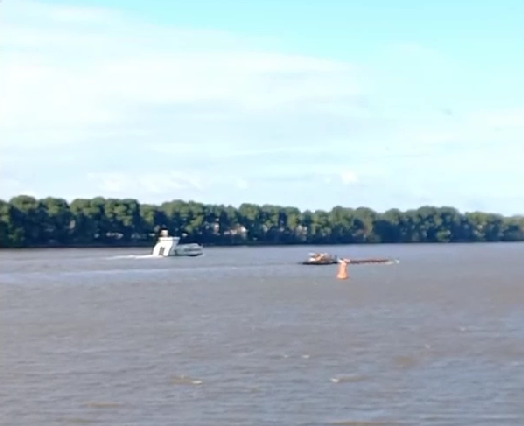
\includegraphics[width=\textwidth]{images/Evaluation/shiptracking_raw.png}
			\caption{Screenshot aus Beispieldatensatz Schiffstracking}
		\end{subfigure} \hfill
		\begin{subfigure}[b]{0.45\textwidth}
			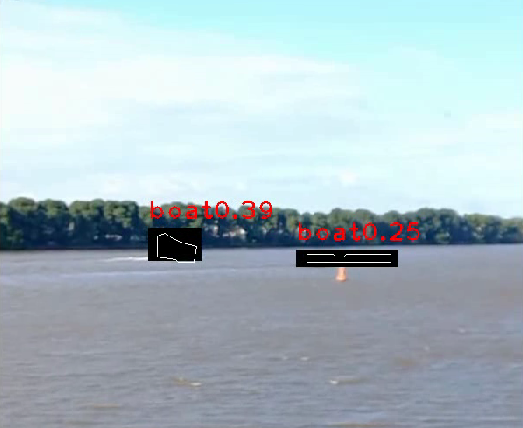
\includegraphics[width=\textwidth]{images/Evaluation/shiptracking_analyzed.png}
			\caption{Screenshot aus analysiertem Beispieldatensatz Schiffstracking}
		\end{subfigure}
		\caption[Screenshots zu Testdatensatz für Schiffstracking]{Screenshots zu Testdatensatz für Schiffstracking. (a) zeigt die Testdaten ohne Bearbeitung; (b) zeigt den Frame mit YOLO analysiert und von der DCE vereinfacht (Quelle: eigene Darstellung)}
		\label{Scr:Testdatensatz_Shiptracking}
	\end{figure} In Tabelle \ref{tab:Shiptracking_Analysis} ist der Vergleich der statistischen Daten zwischen den beiden verschieden langen Videos zu sehen. Auffällig ist, dass die durchschnittliche Abweichung pro Polygon deutlich absinkt, während die Abweichung pro Winkel steigt. Dies lässt sich mit den hohen Punktwerten nach der DCE erklären, aber auch damit, dass durch die Boje aus einem Schiff mehrere Schiffe von YOLO detektiert worden sind. Dies sorgt für eine hohe Abweichung, da die Boje den Umriss stark verfälscht. \\
	Die absolute Abweichung steigt bei dem längeren Video um ca. das 13-fache an. Dies kann mit der höheren Frameanzahl erklärt werden, wie auch die Zahl der erkannten Punkte/Winkel und Polygone, sowie der deutlich höheren Zahl der verglichenen Polygone. \\
	Die Prozessierungszeit von YOLO verdoppelt sich durch die höhere Framezahl, die Dauer der DCE steigt hingegen durch die erhöhte Anzahl von Polygonen deutlich stärker an. Beides ist dann auch in der Gesamtdauer des Programmes zu erkennen. \\
	Die SSM pro Klasse sinkt mit der höheren Framezahl ab, da mehr erkannte Polygone bei gleichbleibender Punktzahl zu einer Verringerung von diesem Wert führen. Dies ist auch deutlich bei der SSM pro detektiertes Boot zu erkennen, die ca. um die Hälfte verringert ist. \\

	\begin{table}[ht]
		\centering
		\caption[Auswertung Schiffstracking Datensatz]{Auswertung Schiffstracking Datensatz; S1s ist der 1-sekündige Datensatz, S21s ist der 21-sekündige Datensatz (Quelle: eigene Darstellung; \ref{cd:listing_A1s_RV_shiptracking_results.txt(Y8x)}, \ref{cd:listing_A21s_RV_shiptracking_results.txt(Y8x)})}
		\label{tab:Shiptracking_Analysis}
		\begin{tabular}{l|l|l|l}
			& \textbf{S1s\_Y8x} & \textbf{S21s\_Y8x} & \textbf{Faktor} \\ \hline
		   \textit{\begin{tabular}[c]{@{}l@{}}Durchschn. Abw.\\ p. Polygon (in Deg.)\end{tabular}} & 48,5 & 29,85 & 0,62 \\ \hline
		   \textit{\begin{tabular}[c]{@{}l@{}}Durchschn. Abw.  \\ p. Winkel (in Deg.)\end{tabular}} & 5,2 & 30,8 & 5,92 \\ \hline
		   \textit{} &  &  &  \\ \hline
		   \textit{\begin{tabular}[c]{@{}l@{}}absolute Abw. \\ (in Deg)\end{tabular}} & 2909,95 & 39109,72 & 13,44 \\ \hline
		   \textit{erk. Punkte/Winkel} & 560 & 12683 & 22,65 \\ \hline
		   \textit{erk.  Polygone} & 60 & 1310 & 21,83 \\ \hline
		   \textit{\begin{tabular}[c]{@{}l@{}}verglichene\\ Polygone\end{tabular}} & 49 & 1213 & 24,80 \\ \hline
			&  &  &  \\ \hline
		   \textit{\begin{tabular}[c]{@{}l@{}}Prozessierungszeit\\ (in Sek.)\end{tabular}} & 33,88 & \begin{tabular}[c]{@{}l@{}}738,25\\ (12,3 Min.)\end{tabular} & 21,80 \\ \hline
		   \textit{Dauer YOLO (in Sek)} & 30,09 & \begin{tabular}[c]{@{}l@{}}602,34\\ (10,04 Min.)\end{tabular} & 2,00 \\ \hline
		   \textit{Dauer DCE (in ms)} & 2,31 & 129,6 & 56,10 \\ \hline
			&  &  &  \\ \hline
		   \textit{SSM pro Fr. und Kl. Boot} & 229,32 & 133,15 & 0,06 \\ \hline
		   \textit{SSM pro detektiertes Boot} & 118,61 & 65,26 & 0,55 \\ \hline
		   \textit{\begin{tabular}[c]{@{}l@{}}Absolute Anz. detektierter\\ Boote (in Klam. pro Fr.)\end{tabular}} & \begin{tabular}[c]{@{}l@{}}58 \\ (1,93)\end{tabular} & \begin{tabular}[c]{@{}l@{}}1310\\ (2,04)\end{tabular} & \begin{tabular}[c]{@{}l@{}}22,59 \\ (1,06)\end{tabular}
		   \end{tabular}
		\end{table}
       \todo{Abschluss finden?}



}
\subsection{Geringe und hohe DCE Substitution}
	{ \todo{tabelen mit quellen versehen!}
		Bei diesem Testdaten werden die Fälle betrachtet, bei denen DCE geringere und höhere Punktgrenzen beachten muss. Als Referenz wird der 8x Datensatz in der Länge 1 Sekunde und in der Länge 10 Sekunden genutzt. Es wird immer die RV Version der Implementierung betrachtet. Die DCE Grenzen sind in Tabelle \ref{tab:YOLO8_minor_more_DCE_Limits} aufgelistet. \\
	\begin{table}[ht]
		\caption{Einstellungen der verschiedenen DCE Substitutionsgrenzen (Quelle: eigene Darstellung; \ref{cd:listing_A1s_RV_minor_results.txt(Y8x)}, \ref{cd:listing_A1s_RV_more_results.txt(Y8x)}, \ref{cd:listing_A10s_RV_minor_results.txt(Y8x)}, \ref{cd:listing_A10s_RV_more_results.txt(Y8x)})}
		\label{tab:YOLO8_minor_more_DCE_Limits}
		\centering
		\begin{tabular}{l|l|l|l}
		 & \textbf{\begin{tabular}[c]{@{}l@{}}Geringe DCE\\ Punktgrenzen\end{tabular}} & \textbf{Referenz} & \textbf{\begin{tabular}[c]{@{}l@{}}hohe DCE\\ Punktgrenzen\end{tabular}} \\ \hline
		\textit{Kl. Auto} & 5 & 10 & 60 \\ \hline
		\textit{Kl. Motorrad} & 3 & 5 & 25 \\ \hline
		\textit{Kl. LKW} & 4 & 8 & 40 \\ \hline
		\textit{anderes Objekt} & 5 & 20 & 100
		\end{tabular}
		\end{table}
		In Tabelle \ref{tab:YOLO8_minor_more_DCE_A1s} ist zu sehen, dass die durchschnittliche Abweichung pro Polygon und Winkel bei geringeren Punktgrenzen stark absinkt und bei höheren Punktgrenzen stark ansteigt. Dies kann man auch auf die absolute Abweichung und die erkannten Punkte übertragen. Da die Zahl der erkannten Punkte steigt, wenn die DCE weniger Punkte entfernt, steigen auch die anderen Werte. Dies gilt auch analog dafür, wenn die DCE mehr Punkte entfernt. \\
		Ein ähnliches Phänomen ist bei der Tabelle \ref{tab:Minor_More_DCE_SSMs_A1s} zu erkennen, wo die SSMs aufgelistet sind. Hier steigt die SSM massiv an, wenn DCE Grenzen angehoben werden und analog dazu sinkt die SSM, wenn die DCE Grenzen verringert werden. Dies ist gleichbleibend bei der absoluten Anzahl der beiden betrachteten Klassen Auto und LKW. \\
		Für die Ergebnisse bei dem 10-sekündigen Video siehe die Tabellen \ref{tab:Minor_More_DCE_SSMs_A10s} (S. \pageref{tab:Minor_More_DCE_SSMs_A10s})  und  \ref{tab:YOLO8_minor_more_DCE_A10s} (S. \pageref{tab:YOLO8_minor_more_DCE_A10s})  im Anhang. Diese Ergebnisse sind auf die oben beschriebenen übertragbar, außer das alle Werte deutlich ansteigen. \\

		\begin{table}[ht]
			\centering
			\caption{Vergleich der Statistik bei 1 Sekunde Video (30 Frames) und verschiedenen DCE Substitutionsgrenzen (Quelle: eigene Darstellung; \ref{cd:listing_A1s_RV_minor_results.txt(Y8x)}, \ref{cd:listing_A1s_RV_more_results.txt(Y8x)})}
			\label{tab:YOLO8_minor_more_DCE_A1s}
			\begin{tabular}{l|l|l|l}
				& \textbf{\begin{tabular}[c]{@{}l@{}}geringe DCE\\ Punktgrenzen\end{tabular}} & \textbf{Referenz} & \textbf{\begin{tabular}[c]{@{}l@{}}hohe DCE\\ Punktgrenzen\end{tabular}} \\ \hline
			   \textit{\begin{tabular}[c]{@{}l@{}}Durchschn. Abweichung\\ p. Polygon (in Deg.)\end{tabular}} & 3,08 & 48,12 & 454,81 \\ \hline
			   \textit{\begin{tabular}[c]{@{}l@{}}Durchschn. Abweichung  \\ p. Winkel (in Deg.)\end{tabular}} & 0,68 & 5,46 & 24,18 \\ \hline
			   \textit{} &  &  &  \\ \hline
			   \textit{\begin{tabular}[c]{@{}l@{}}absolute Abweichung  \\ (in Deg)\end{tabular}} & 658,93 & 10298,28 & 97329,43 \\ \hline
			   \textit{erkannte Punkte/Winkel} & 966 & 1885 & 4026 \\ \hline
			   \textit{erkannte Polygone} & 214 & 214 & 214 \\ \hline
			   \textit{verglichene Polygone} & 194 & 194 & 194 \\ \hline
			   \textit{Prozessierungszeit (in Sek.)} & 107,77 & 102,46 & 80,39
			   \end{tabular}
			\end{table}

			\begin{table}[ht]
				\caption{Vergleich der SSMs bei verschiedenen DCE Substitionslimits bei einem 1-sekündigem Video (30 Frames) (Quelle: eigene Darstellung; \ref{cd:listing_A1s_RV_minor_results.txt(Y8x)}, \ref{cd:listing_A1s_RV_more_results.txt(Y8x)})}
				\label{tab:Minor_More_DCE_SSMs_A1s}
				\centering
				\begin{tabular}{l|l|l|l}
				 & \textbf{\begin{tabular}[c]{@{}l@{}}geringe DCE\\ Punktgrenzen\end{tabular}} & \textbf{Referenz} & \textbf{\begin{tabular}[c]{@{}l@{}}hohe DCE\\ Punktgrenzen\end{tabular}} \\ \hline
				\textit{SSM pro Fr. und Kl. Auto} & 3,12 & 355,41 & 6638,88 \\ \hline
				\textit{SSM pro detektiertes Auto} & 0,90 & 102,52 & 1915,06 \\ \hline
				\textit{\begin{tabular}[c]{@{}l@{}}absolute Anz. detektierter\\ Autos (in Klam. pro Fr.)\end{tabular}} & 104 (3,47) & 104 (3,47) & 104 (3,47) \\ \hline
				 &  &  &  \\ \hline
				\textit{SSM pro Fr. und Kl. LKW} & 39,52 & 14,19 & 10388,78 \\ \hline
				\textit{SSM pro detektierter LKW} & 11,40 & 4,09 & 2996,76 \\ \hline
				\textit{\begin{tabular}[c]{@{}l@{}}absolute Anz. detektierter\\ LKW (in Klam. pro Fr.)\end{tabular}} & 104 (3,47) & 104 (3,47) & 104 (3,47)
				\end{tabular}
				\end{table}		
	 }
	 \clearpage
\subsection{lange Testdatensätze (NICHT FERTIG)}{
	\todo{müssen noch gemacht werden }
}
{
	

}
% 	\section{Bewertung}
% 	{ %Zusammenfassen kann man sagen, dass die durchschnittliche Abweichung pro Polygon nach der Vereinfachung von DCE zu hoch ist, um ein Tracking zu ermöglichen. Beim Einsatz der größeren Modelle steigt die Winkelabweichung und SSM an, dies ist aber zu vernachlässigen, da die Klassifizierung der Objekte genauer erfolgt. Insbesondere der Vergleich der SSM innerhalb einer Klasse  ist die Abweichung sehr hoch. \\
% 	%Die Implementierung der YOLO Version in der Variante, dass das Video in einzelne Frames zerlegt wird und diese einzeln analysiert werden, hat sich im Vergleich zur direkten vollständigen Analyse mit YOLO als zu ineffektiv herausgestellt und kann damit verworfen werden. 
	
% 	Zusammenfassen kann man sagen, dass die durchschnittliche Abweichung pro Polygon nach der Vereinfachung von DCE gering genug ist, um ein Tracking zu ermöglichen. Beim Einsatz der größeren Modelle steigt die Winkelabweichung und SSM an, dies ist aber zu vernachlässigen, da die Klassifizierung der Objekte genauer erfolgt.  \\
% 	Die Implementierung der YOLO Version in der Variante, dass das Video in einzelne Frames zerlegt wird und diese einzeln analysiert werden, hat sich im Vergleich zur direkten vollständigen Analyse mit YOLO als zu ineffektiv herausgestellt und kann damit verworfen werden. }

% \section{Ausblick}
%  { 
% %	\begin{enumerate}
% % 	\item DCE Abbruchbedingung nicht fest implementieren sondern einen Wert einführen, der immer im Vergleich zur Ähnlichkeit des Ursprungspolygons gemessen wird. Ermöglicht eine bedarfsbezogene Vereinfachung des Polygons, individuell für jeden erkannten Umriss
% % 	\item Implementierung der DCE; bzw. anderer Programmteile in schnellerer Programmiersprache wie C/C++; bzw. hardwarenah(er)
% % \end{enumerate}
	


% }



